\documentclass[amsmath,amssymb, aps, prx, longbibliography, twocolumn]{revtex4-1}

\usepackage{natbib}
\usepackage{graphicx}% Include figure files
\usepackage{dcolumn}% Align table columns on decimal point
\usepackage{bm}
\usepackage[usenames]{color}

\begin{document}

%\title{Machine learning transport with quantum loop topography}
\title{ Probing transport in quantum many-fermion simulations\\ via quantum loop topography}

\author{Yi Zhang$^1$}
\email{frankzhangyi@gmail.com}
\author{Carsten Bauer$^2$}
\author{Peter Broecker$^2$} 
\author{Simon Trebst$^2$}
\author{Eun-Ah Kim$^1$}
\email{eun-ah.kim@cornell.edu}

\affiliation{%
$^{1}$Department of Physics, Cornell University, Ithaca, New York 14853, USA}%
\affiliation{$^{2}$Institute for Theoretical Physics, University of Cologne, 50937 Cologne, Germany}

\date{\today}% It is always \today, today,
             %  but any date may be explicitly specified

\begin{abstract}
Quantum many-fermion systems give rise to diverse states of matter that often reveal themselves in distinctive transport properties. While some of these states can be captured by microscopic models accessible to numerical exact quantum Monte Carlo simulations, it nevertheless remains challenging to  numerically access their transport properties. 
Here we demonstrate that quantum loop topography (QLT) can be used to directly probe transport by machine learning current-current correlations in imaginary time.
We showcase this approach by studying the emergence of superconducting fluctuations in the negative-U Hubbard model and  
an effective action model for a metallic %n antiferromagnetic
quantum critical point. 
For both sign-free models we find that the QLT approach detects a change in transport in very good agreement with their established 
phase diagrams.
%derived from conventional numerical estimators.
These proof-of-principle calculations combined with the numerical efficiency of the QLT approach point a way to identify hitherto elusive
transport phenomena such as non-Fermi liquids using machine learning algorithms.
\end{abstract}

\maketitle

%%%%%%%%%%%%%%%%%%%%%%%%%%%%%%%%%%%%%%%%%%%%%%%%%%%%%%%%%%%%%%%%%%
% Introduction
%%%%%%%%%%%%%%%%%%%%%%%%%%%%%%%%%%%%%%%%%%%%%%%%%%%%%%%%%%%%%%%%%%

Quantum many-body systems exhibit an intriguing diversity of collective states that have no classical counterpart.
Paradigmatic examples include the formation of Bose-Einstein condensates and superfluids in bosonic systems, 
the emergence of spin liquids and macroscopic entanglement in magnetic systems, 
or the observation of superconductivity in many-electron systems. 
But while the microscopic physics giving rise to these phenomena are well understood for systems 
of many interacting bosonic or spin degrees of freedom, 
either via controlled analytical calculations for minimal model Hamiltonians or via numerical simulations
providing even quantitative guidance, the fundamental understanding of quantum many-fermion systems
has proved to be more elusive. The distinct feature leading to a seemingly unsurmountable complication
for these systems arguably is the profusion of gapless modes near the Fermi energy. 
On the analytical side, the concurrent treatment of these gapless modes and their interactions with other (bosonic) soft modes,
e.g.~in the vicinity of a quantum phase transition \cite{Hertz1976,Millis1993}, has remained a formidable challenge.
On the numerical side, many-fermion systems have long proved to resist a solution via quantum Monte Carlo techniques
due to the occurrence of the so-called sign problem that is closely linked to the complex sign structure of the 
many-fermion wavefunction (another consequence of the existence of a multitude of gapless modes).
Adding to this complexity, the key features revealing the nature of collective many-fermion states 
(such as superconductors, strange metals, or non-Fermi liquids) are often their transport properties
that are notoriously difficult to calculate.   


It is the purpose of this manuscript to outline a numerical scheme that 
allows for a direct quantitative probe of transport properties in interacting many-electron systems
by combining elements from machine learning and quantum Monte Carlo (QMC)
techniques. 
To do so, we build on progress on two separate fronts advancing the numerical description of many-fermion systems.
First, it has been realized that quantum criticality in itinerant fermion systems can be studied in a numerically exact manner 
in sign-problem free models 
\cite{Berg2012,Schattner2016a,Gerlach2017,Xu2017a,Lederer2017,Li2016,Li2017,Jiang2017,Berg2018}
built around the effective action for multiple fermion bands. 
However, to infer transport properties one faces the problem that QMC simulations intrinsically yield imaginary time data, 
and the analytic continuation of imaginary time data to real time is numerically ill posed, yielding no controlled framework
to probe transport properties. 
Instead, we resort to the recent development of machine learning approaches in quantum statistical physics and demonstrate that quantum loop topography (QLT), a numerical scheme initially designed to identify the topological Hall response of a system~\cite{qlt2016}, can in fact be used to measure {\em longitudinal} transport properties of itinerant many-fermion systems.

Here we show that the QLT approach can be adapted to extract the essential features from the imaginary time current-current correlation function, readily available from QMC simulations. One principle example which we focus on is the study of superconductivity, whose onset can, in principle, be tracked e.g. via the superfluid density that can be rigorously obtained starting from current-current correlation function \cite{Scalapino1992,Scalapino1993}. 
Here we show that the QLT+QMC approach succeeds in identifying the essential features of this transition without any prior knowledge (e.g. about the explicit calculation of the superfluid density)
and quantitatively matches existing results for the superconducting transition for a number of microscopic model systems,
but at considerably lower computational cost.






%Key challenge with studying quantum many-fermion systems has to do with the fact that the defining macroscopic characteristic of a state is often its transport property. Unfortunately, 
%rigorous information on transport one can gain from Monte Carlo simulations is limited because Monte Carlo simulations yield imaginary time data, and the analytic continuation of imaginary time data to real time is numerically ill posed. Nevertheless, the imaginary time current-current correlation function must contain the nugget of the key information regarding transport. Indeed 
%superfluid density can be rigorously obtained to signal superconductivity\cite{Scalapino1992,Scalapino1993} and even a “proxy” for the DC resistivity can be obtained to hint at non-Fermi liquid behavior\cite{Lederer2017}, all starting from current-current correlation function. Therefore it is plausible that a machine learning approach that targets information relevant for current-current correlation can enable efficient acquisition of phase diagrams by probing qualitative change in transport.
%
%{\color{red} (Simon: We need to go from many-fermion to QMC. We may not want to bring in quantum criticality.)} Quantum criticality with itinerant fermions can be studied exactly in sign-problem free models that are nevertheless quite rich \cite{Berg2012,Schattner2016a,Gerlach2017,Xu2017a,Lederer2017,Li2016,Li2017,Jiang2017,Berg2018}, motivating interest in studying phase diagrams of variety of  “sign-free” models. Nevertheless, ``sign-free'' does not imply ready accessible. 
%In fact, scanning the multi-dimensional phase space can be quite time-consuming, even if the absence of the sign problem makes the cooling down to low-temperatures possible in principle. One approach to speeding-up Monte Carlo simulations using machine learning is to making each update more efficient by either increasing the acceptance rate using the restricted Boltzmann machines to propose updates\cite{Huang2017}, or finding an approximate Hamiltonian to guide update suggestions\cite{Liu2017}. 
%An alternative is to minimize the number of necessary updates by using the ANN’s ability to “see through” a noisy data. {\color{red} (Simon: a summary of literature here ending with importance of input?)}
%
%
%
%In this paper, we adapt the QLT first introduced in Ref.~\cite{qlt2016} for the topological Hall response to the longitudinal transport.  {\color{red}(EK: a few words on how QLT worked for topological response.)}


%Machine learning techniques have emerged as an effective alternative to big data analysis and regression towards the underlying clues in abstract entities such as images and voices\cite{MLbook}. Recently, machine learning have shown exciting developments in the territories of the condensed matter physics, where similar 'big data' issues have laid increasing challenges in researches. Indeed, methods such as the neural network states\cite{Carleo2016, Deng2016, Deng2017, Glasser2018, Torlai2018, Gaoxun2017} and self-learning simulations\cite{Meng2016, Leiwang2017, Junwei2017b, Junwei2017c} have largely impacted our capacity towards representing quantum many-body states. On the other hand, it is vital to identify the corresponding phases of the many-body states, which characterize the low-energy collective behaviors and dominate their general properties. It is the similarity between this task and the iconic success of machine learning in image recognition that has inspired the rapid progress of applying machine learning techniques to phase recognition\cite{Melko20161, Nieuwenburg2017, LeiWang2016, Simon2016, Kelvin2016, Ohtsuki2016, Ohtsuki2017, Titus2017, qlt2016, FrankMLZ2, Broecker2017, ZhaiHui2017, Iakovlev2018, PollmannML2018, Anna2018}, especially for difficult problems involving strong correlations and topological phases that defies conventional approaches. 
%Superconductivity is the fascinating phenomena of exactly zero electrical resistance and expulsion of magnetic fields. Despite the vast diversity among the conventional phonon-assisted BCS superconductors and the unconventional superconductors such as the Cu-based, Fe-based and heavy-Fermion materials, they are universally characterized by electrons forming Cooper pairs. On the other hand, unlike other Landau symmetry breaking phases, the superconductors break the $U(1)$ gauge symmetry. Except for the mean-field theories that explicitly break the charge conservation, a well-defined order parameter signaling the symmetry breaking is not immediately available for emergent superconductivity. Pair correlation offers a partial substitute yet still decays in two dimensions making identification ambiguous in finite size systems. A more established signature is the advent of a non-zero superfluid density $\rho_s$, obtainable from the longitudinal and transverse current-current correlations\cite{Superfluids, Scalapino1992, Scalapino1993, Nandini1996}. For this purpose, we need to measure the current-current correlations $\Lambda_{xx}$ across the entire real space as well as the imaginary time. This requires a large number of samples in a Monte Carlo simulation in order to suppress the uncertainty, especially for correlations over distances with small expectation values. Then, we Fourier transform, extrapolate to the long-wavelength limits $\omega=0, q_x\rightarrow0, q_y=0$ and $\omega=0, q_x=0, q_y\rightarrow0$, and take the difference. The overall cost for a clear-cut detection of the superconductivity is still rather high, especially near the superconducting transition where the value of $\rho_s$ is small.
%In this paper,  we use supervised machine learning for purpose of detecting emergent superconductivity from interacting fermionic systems.


%Here we consider emergent $s$-wave superconductivity in the negative $U$ Hubbard model\cite{Scalettar1989, Scalapino1992} and the emergent $d$-wave superconductivity in models where the Fermi surfaces are coupled to a $\vec Q=(\pi, \pi)$ spin density wave (SDW) order parameter\cite{Erez2016}. Both models can be simulated via Determinant Quantum Monte Carlo (DQMC) methods without the sign problem. 

%Instead of calculating the superfluid density, we focus on the two-point correlations as our raw data source, which are conveniently available in DQMC calculations. Two artificial neural network (ANN) architectures are applied in parallel: a deep neural network with convolutional layers\cite{Simon2016}, and a shallow neural network with a feature selection layer dubbed as quantum loop topography\cite{qlt2016, FrankMLZ2}, focusing on correlations trailing three-point and four-point loops at the shortest length scales. Both architectures have their respective merits: while the deep convolutional neural network is powerful enough to minimize our human intervention, the introduction of quantum loop topography as humanly inspired by the physical relevance of the information - the current-current correlations in this case - helps to reduce the complexity of the ANN and the corresponding efforts for supervised machine learning. We train our artificial neural networks with data deep in the superconducting phases at low temperature and normal phase at high temperature. Benchmarks suggest that in both scenarios we can achieve good performance with a small number of uncorrelated Monte Carlo samples, therefore largely reduce the computational cost of the conventional algorithm. 
%Although our examples are two-dimensional models, it is straightforward to generalize the methods to other dimensions. 

%%%%%%%%%%%%%%%%%%%%%%%%%%%%%%%%%%%%%%%%%%%%%%%%%%%%%%%%%%%%%%%%%%
% Quantum loop topography for longitudinal transport
%%%%%%%%%%%%%%%%%%%%%%%%%%%%%%%%%%%%%%%%%%%%%%%%%%%%%%%%%%%%%%%%%%


%\section{Quantum loop topography for longitudinal transport}
\noindent{\em QLT for longitudinal transport.-- }
The recent foray of applying machine learning techniques to quantum many-body systems can roughly be divided into two classes of general approaches: 
(i) the representation of many-body wavefunctions using restricted Boltzmann machines allowing for a new class of variational algorithms to efficiently find ground states of quantum many-body systems
\cite{Carleo2016, Deng2016, Deng2017, Glasser2018, Torlai2018, Gaoxun2017}, and 
(ii) the use of artificial neural networks, typically combined with preprocessing steps, to allow for quantum state recognition 
\cite{Melko20161, Nieuwenburg2017, LeiWang2016, Simon2016, Kelvin2016, Ohtsuki2016, Ohtsuki2017, Titus2017, qlt2016, FrankMLZ2, Broecker2017, ZhaiHui2017, Iakovlev2018, PollmannML2018, Anna2018}.
%
In the latter category, the QLT approach~\cite{qlt2016} stands out as a preprocessing step that selects and organizes the simulation data with the {\em physical response} characteristic of the target phase in mind (and thereby distinguishes itself from e.g.~the application of convolutional neural networks whose motivation is primarily rooted in image recognition techniques). The QLT approach has so far been successfully employed for topological phases by targeting Hall transport for the integer and fractional Chern insulators~\cite{qlt2016} and targeting Wilson loops for $\mathbb{Z}_2$ spin liquid~\cite{Zhang2017}.
%{\color{red}(ST: Eun-Ah, please add a few words on how QLT worked for topological response.)}
%

Targeting the longitudinal transport for the purpose of the current study, we build a vector at each site $j$ consisting of all small loops with three vertices, $L^\triangle_{jkl}$ and with four vertices, $L^\Box_{jklm}$ including the site $j$. The loops represent
chained products of bilinear fermionic operators  $c_i^\dagger c_j^{\phantom\dagger}$ evaluated for a given Monte Carlo sample 
$\alpha$, $\widetilde{P}_{jk}|_{\alpha}$:
\begin{equation}
    L^\triangle_{jkl}\equiv\widetilde{P}_{jk}|_{\alpha} \widetilde{P}_{kl}|_{\beta} \widetilde{P}_{lj}|_{\gamma} \,,
    \label{eq:triangle}
\end{equation}
and 
%limiting the neighboring sites to be within a short-distance cutoff $d_c$. 
%Now in order to target the longitudinal transport, in addition to the triangular loops %$L^\triangle_{jkl}$ in Eq.~\ref{eq:triangle}, we use quadralateral loops $L^\Box_{jklm}$:
\begin{equation}
L^\Box_{jklm}\equiv\widetilde{P}_{jk}|_{\alpha'} \widetilde{P}_{kl}|_{\beta'} \widetilde{P}_{lm}|_{\gamma'} \widetilde{P}_{mj}|_{\delta'} \,,
\label{eq:quad}
\end{equation}
limiting the neighboring sites to be within a short-distance cutoff $d_c$. 
The loop operators associated with a site are illustrated in Fig.~\ref{fig:loops} for the shortest lengths, i.e. length 3 and 4.

\begin{figure}[b]
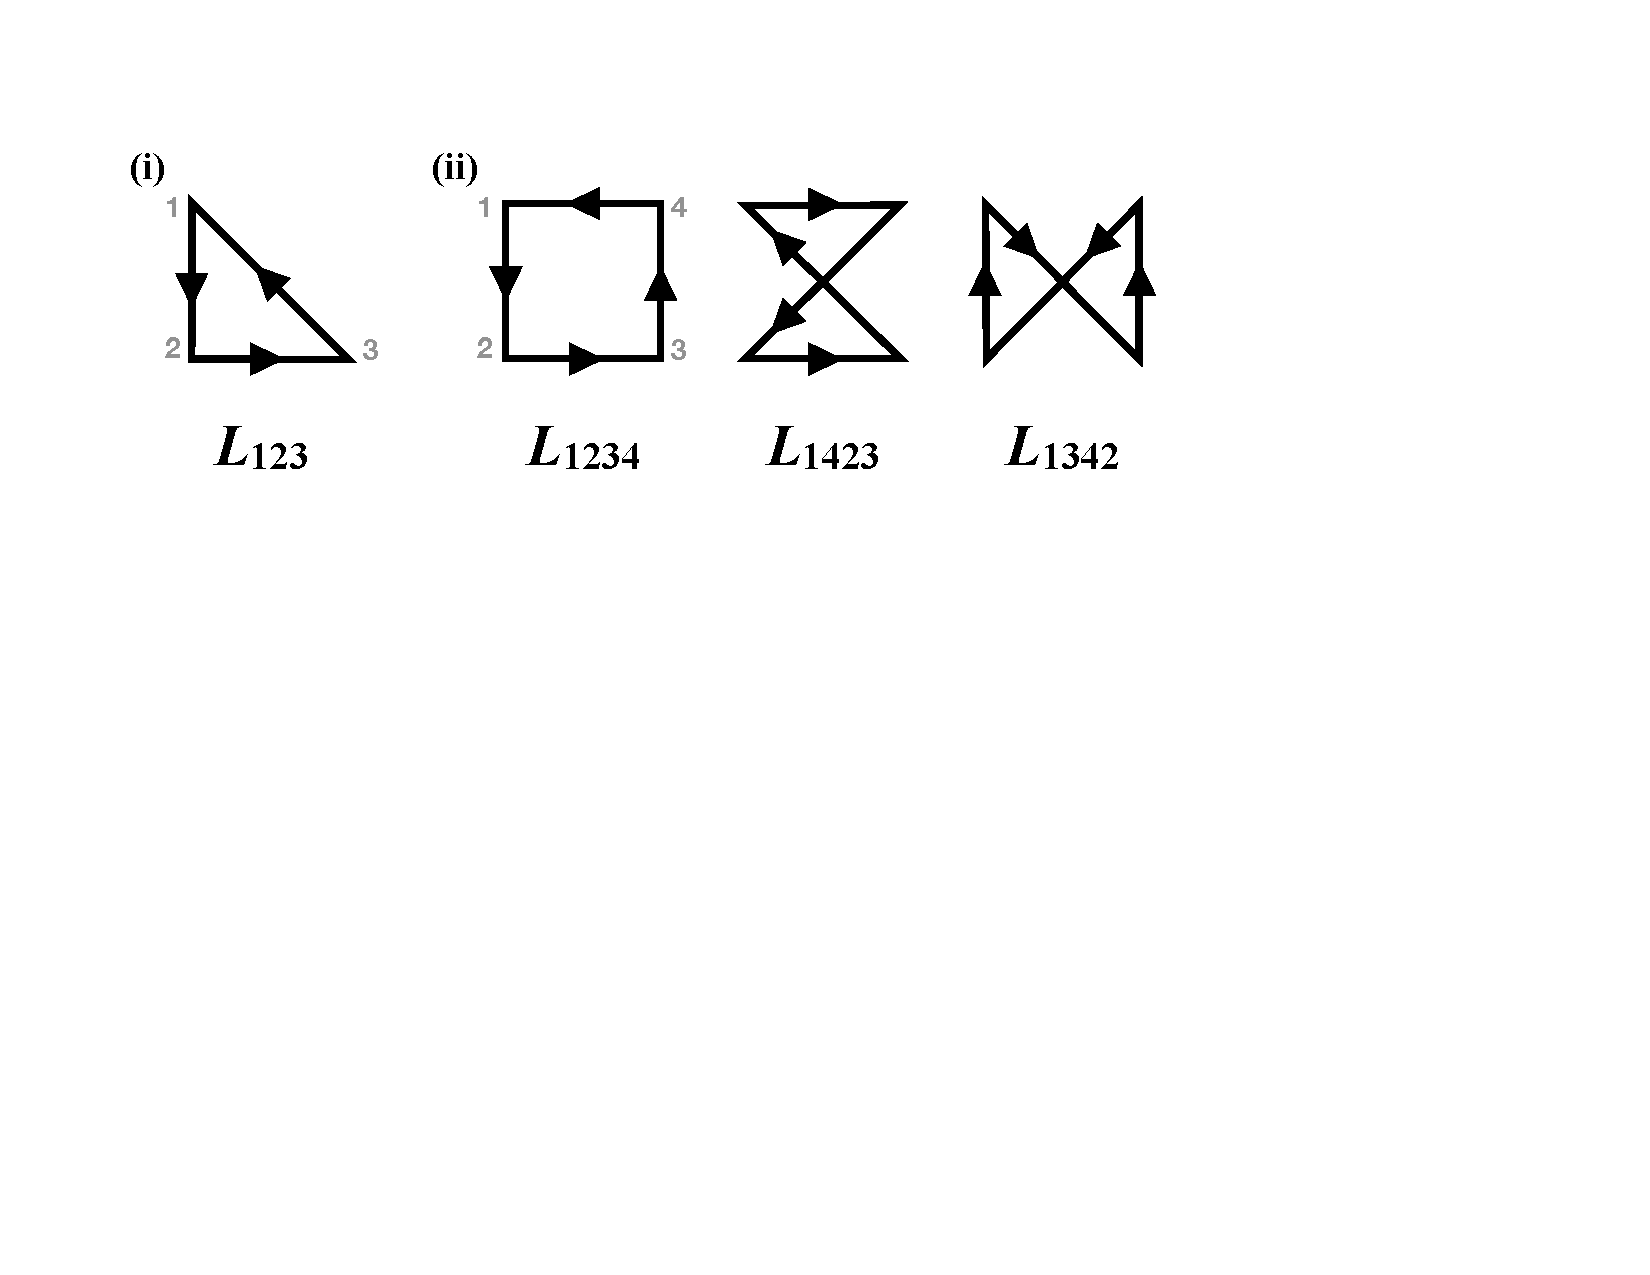
\includegraphics[scale=0.48]{LoopOperators.pdf}
\caption{
 Illustration of the (i) triangular and (ii) quadralateral {\bf loop operators} employed to calculate the longitudinal transport. 
}\label{fig:loops}
\end{figure}

To see how the loop operators $L^\Box_{jklm}$ and $ L^\triangle_{jkl}$ capture the longitudinal transport, consider the zero-frequency current-current correlation function:  
\begin{equation}
\Lambda_{xx}({\bf r}_1,{\bf r}_2;\omega_n=0)\equiv\int d\tau\left\langle \hat{j}_x\left({\bf r}_1, \tau \right) \hat{j}_x\left({\bf r}_2, 0 \right)\right\rangle,
\label{eq:Lambda}
\end{equation}
where $\hat{j}_x({\bf r}_1,\tau)=e^{\hat{H}\tau} \hat{j}_x({\bf r}_1) e^{-\hat{H}\tau}$ with the current density operator $\hat{j}_x({\bf r_1})= -i[\hat{H}({\bf r}_1),\hat{x}]$. The Fourier transform of the 
current-current correlation function in Eq.~\eqref{eq:Lambda} is famously related to the superfluid density $\rho_s$ through $\rho_s\propto \Lambda_{xx}(q_x\!\rightarrow\! 0,q_y\!=\!0,\omega_n\!=\!0)-\Lambda_{xx}(q_x\!=\!0,q_y\!\rightarrow\!0,\omega_n\!=\!0)$ \cite{Scalapino1993, Scalapino1992}. 
%$\left|G\right\rangle$ is the target ground state. 
%Given the imaginary time evolution $j_x(r_1,\tau)=e^{H\tau} j_x(r_1) e^{-H\tau}$,
%\begin{eqnarray}
%& &\int d\tau \left\langle j_x\left(r_1, \tau\right) j_x\left(r_2, 0 \right)\right\rangle
%\nonumber\\
%&=&\sum_{n\ne G} \frac{\left\langle G \left| j_x(r_1)  \left|n\left\rangle  \right\langle n\right| j_x(r_2)\right| G\right\rangle}{E_n-E_G}.
%\label{eq:lambdaform}
%\end{eqnarray}
To make further progress analytically, consider 
%Now a rigorous relationship between the Loop operators $L^\Box_{jklm}$ and $ L^\triangle_{jkl}$  and the longitudinal current response can be established for
a gapped mean-field Hamiltonian which can approximated as $\hat{H}'=-\hat{P}$ with flat band, where
%For a gapped Hamiltonian, the Hamiltonian can be approximated by a flat band Hamiltonian  $H'=-\hat{P}$  with the 
%if we consider
%the projection operator
$\hat{P}\equiv |G\rangle \langle G|$ is the projection operator for the ground state $|G\rangle$. At zero temperature we can evaluate the current-current correlation function for the system with the Hamiltonian $\hat{H}'$:
%, the right hand side of Eq.~\ref{eq:lambdaform} simplifies to 
%and approximate the Hamiltonian $H'=-P$. $H'$ is adiabatically connected to $H$ in the gapped phase yet it has a simpler flat excitation spectrum $E_n-E_G=1$. Now 
%\begin{eqnarray}
    %\sum_{n\ne G} \frac{\left\langle G \left| j_x(r_1)  \left|n\left\rangle  \right\langle n\right| j_x(r_2)\right| G\right\rangle}{E_n-E_G}
   %\Lambda_{xx}({\bf r}_1,{\bf r}_2;\omega_n\!=\!0) &=& \langle G|j_x({\bf r}_1)(1-\hat{P}) j_x({\bf r}_2)|G\rangle \nonumber\\
  % &=&{\rm Tr}\ \left[\hat{P}j_x({\bf r}_1)(1-\hat{P}) j_x({\bf r}_2)\right],
%\end{eqnarray}
%where we set the gap energy scale to be 1.
%where we have suppressed the position arguments. 
%Inputting the expression for $j_x({\bf r})$, the trace can be evaluated to be
%urther using the fact that current density is given by the commutator of the Hamiltonian and the position operator, we obtain
\begin{equation}
%P j_x \left(1-P\right) j_x &=& - P \left[H',x\right] \left(1-P\right) \left[H',x\right] \nonumber\\
\left. \begin{aligned}
\Lambda_{xx}(&{\bf r}_1,{\bf r}_2;\omega_n\!=\!0)
= \langle G|\hat{j}_x({\bf r}_1)(1-\hat{P}) \hat{j}_x({\bf r}_2)|G\rangle \\
   &={\rm Tr}\ \left[\hat{P}\hat{j}_x({\bf r}_1)(1-\hat{P}) \hat{j}_x({\bf r}_2)\right],\\
&= \sum_{{\bf r}_3 {\bf r}_4}P_{{\bf r}_2 {\bf r}_4}P_{{\bf r}_4{\bf r}_1}P_{{\bf r}_1{\bf r}_3}P_{{\bf r}_3{\bf r}_2}\left(x_1-x_4\right)\left(x_2-x_3\right) \\
& \quad - \sum_{{\bf r}_4}P_{{\bf r}_2 {\bf r}_4}P_{{\bf r}_4{\bf r}_1}P_{{\bf r}_1{\bf r}_2}\left(x_1-x_4\right)\left(x_2-x_1\right) \,,
\end{aligned}
\right.
\label{eq:j-j}
\end{equation}
where $P_{{\bf r}'{\bf r}}\equiv \langle G|c^\dagger_{{\bf r}'} c_{\bf r}|G\rangle $ is the two-point function and $x_i$ is the $x$ coordinate of position ${\bf r}_i$. Here, we used the definition of the current density operator for the third equality~\footnote{For a Bogoliubov deGenne Hamiltonian, $H'$ takes the fermion bi-linear form after relabelling a set of fermion annihilation operators as creation operators and vice versa.}.
(See Appendix for further detail.)
Hence for the approximate Hamiltonian $\hat{H}'$ at zero temperature, the current-current correlation function consists of an appropriately weighed combination of quadrilateral loops and triangular loops of two-point functions.

Note that  $L^\triangle_{jkl}$ and  $L^\Box_{ijkl}$ defined in Eqs.~\eqref{eq:triangle} and \eqref{eq:quad} involves samples of the Green's functions $\widetilde{P}_{jk}|_{\alpha}$ typically coming from a determinant quantum Monte Carlo (DQMC) calculation. 
By processing the loop operators during the sampling process and avoiding an a posteriori Monte Carlo averaging, we quickly pass these fluctuation-laden data which should encode information of current-current correlation function, to the machine learning step. 
%Since NN's can learn to form the relevant combination of the inputs we use both $L^\triangle_{jkl}$ and  $L^\Box_{ijkl}$ defined in Eqs.~\ref{eq:triangle} and \ref{eq:quad} as inputs. 
%Note that we use Determinent quantum Monte Carlo (DQMC) samples of the Green's functions $\widetilde{P}_{jk}|_{\alpha}$. Such data is intrinsically fluctuation-laden, yet it allows us to generate abundant samples for a given model, and at the same time reduces the computation cost by reducing the number of necessary updates\cite{qlt2016, FrankMLZ2, Simon2016, Kelvin2016}. After the ANN is trained and optimized with samples from low and high temperatures with the pre-existing labels, the resulting ANN is used to identify the superconducting transport at intermediate temperatures based upon their respective DQMC samples.  
Clearly, the loop operators $L^\Box_{jklm}$ and $ L^\triangle_{jkl}$ built from single Monte Carlo instances and only for short-ranged loops, cannot replace a rigorous calculation of the current-current correlation function, especially for a gapless system. But we anticipate the QLT consisting of the triangular and quadrilateral loops to serve as a  proxy for the current-current correlation function containing qualitative information regarding longitudinal transport directly in the imaginary time data.  

%Since NN's can learn to form the effective combination of the inputs, Eq.~\ref{eq:j-j} suggests that use of both $L^\triangle_{jkl}$ and  $L^\Box_{ijkl}$ defined in Eqs.~\ref{eq:triangle} and \ref{eq:quad} as inputs could enable ANN's to probe transport properties in imaginary time data. Throughout the rest of this paper we focus on only the loops with the smallest length scales, since the correlation $P$ decays over distances. For the rest of the paper, we only include the quantum loops $L$ and $L'$ whose width is equal or below a cut-off scale $d_c=2$ unless noted otherwise.


%%%%%%%%%%%%%%%%%%%%%%%%%%%%%%%%%%%%%%%%%%%%%%%%%%%%%%%%%%%%%%%%%%
% Models and Results
%%%%%%%%%%%%%%%%%%%%%%%%%%%%%%%%%%%%%%%%%%%%%%%%%%%%%%%%%%%%%%%%%%



%\section{Models and Results}
\noindent{\em Models and Results.-- }
%
To test the potential of the QLT for efficiently detecting qualitative difference in the transport from imaginary time Greens function data, we consider models that host superconductivity in parts of their respective phase diagrams.
There are two subtleties to detecting superconductivity from a simulated data in two spatial dimension (2D). The first subtlety is that superconducting order parameter is not accessible to a simulation that preserves particle number. Hence one must follow the carefully defined limiting process to obtain the superfluid density from current-current correlation function\cite{Scalapino1993, Scalapino1992}. The second subtlety is that superconducting transition in 2D is of Kosterlitz-Thouless (KT) type and hence the superconducting transition is signaled by the superfluid density exceeding the KT critical value\cite{KT1973}. Merely non-zero value of superfluid density instead signals onset of diamagnetism and superconducting fluctuations. Given the explicit tie between the QLT and the zero-frequency current-current correlation function discussed earlier for the simple gapped Hamiltonian, we can anticipate QLT to have enough information on superconducting fluctuations for artificial neural network (ANN) to recognize.  

%{\color{blue}Due to the Kosterlitz-Thouless type transition and the absence of accessible superconducting order parameter in two dimensions, a rigorous characterization within DQMC commonly relies on the calculation of the superfluid density\cite{Scalapino1993, Scalapino1992, Nandini1996}. While a non-zero superfluid density signals the onset of diamagnetism thus the existence of superconducting fluctuation\cite{Erez2016}, the actual onset of the superconducting order requires the superfluid density to surpass certain value proportional to the transition temperature\cite{KT1973}.}
%A rigorous detection of the onset of superconductivity requires XXX within DQMC since the superconducting order parameter itself is not directly accessible in DQMC which conserves particle number by construction. One can also do YYY to detect the existence of superconducting fluctuation.

We first consider the prototypical model with superconductivity: the negative $U$ Hubbard model on a two-dimensional square lattice\cite{Scalettar1989, Scalapino1992}. 
\begin{eqnarray}
H &=& H_0 + H_U -  \mu\underset{i}{\sum} \left(n_{i,\uparrow} +n_{i,\downarrow}\right) \nonumber\\
H_0 &=& -\underset{\left\langle ij \right\rangle, s}{\sum} \left( c^\dagger_{j,s}c_{i,s} +  c^\dagger_{i,s}c_{j,s} \right) \nonumber \\
H_U &=& U \underset{i}{\sum} \left(n_{i,\uparrow}-\frac{1}{2}\right) \left(n_{i,\downarrow}-\frac{1}{2}\right)
\label{eq:hubbard}
\end{eqnarray}
where $s = \uparrow, \downarrow$ denotes the spin, $c^\dagger_{i,s}$ is the electron creation operator, and $n_{i,s}=c^\dagger_{i,s}c_{i,s}$ is the electron density operator. $U=-\left|U\right|<0$ is the attractive interaction strength and $\mu$ is the chemical potential. We study the system size of $8\times 8$. Without loss of generality, we set $U=-8$ and the electron density $\left\langle n\right\rangle = \left\langle n_\uparrow\right\rangle+ \left\langle n_\downarrow\right\rangle  \simeq 0.9$ slightly below half filling.  For each site of the lattice, we then build and collect site-touching quantum loops $L^\Box$ and $ L^\triangle$ of linear dimension less than two lattice constants. The QLT so constructed forms the input vector $x$ for the shallow ANN  depicted in Fig.~\ref{fig:network_architecture}.


%After proper Trotter decomposition and mapping the system into 2+1 dimensions with the imaginary time direction controlling the systematic temperature, both models can be simulated via DQMC methods without the sign problem. Both models exhibit a superconductor-metal transition at a critical temperature\cite{Scalettar1989, Scalapino1992,Erez2016}. On the other hand, while the pairing symmetry is naturally $s$-wave in the negative $U$ Hubbard model, the low-temperature superconducting phase of the effective action model in Eq.~\eqref{eq:afmetal} that consists two flavors of fermions coupled to an SDW order parameter and exhibits $d$-wave pairings. 

\begin{figure}
    \centering
    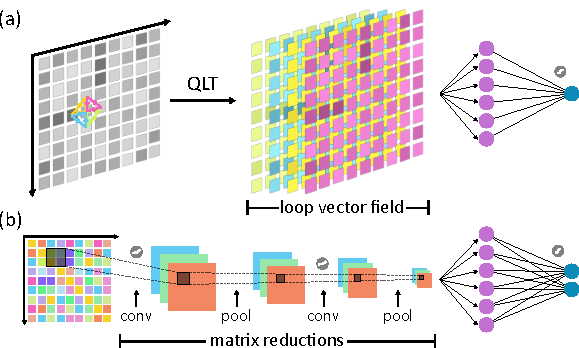
\includegraphics[scale=.85]{architecture.pdf}
    \caption{{\bf Neural network architectures}. 
    			(a) QLT used as an input to a feed-forward fully-connected shallow neural network with one hidden layer 
			consisting of $n=40$ sigmoid neurons. Only triangular loops are illustrated.
			%Each neuron processes the input $x$ through independent weights and biases $w\cdot x+b$. 
    			(b) Deep convolutional neural network that convolves and pooles the unprocessed Green's functions 
				$\widetilde{P}_{jk}|_{\alpha}$ before threading them through a fully-connected layer of $n=256$ hidden neurons.}
    \label{fig:network_architecture}
\end{figure}

%Specifically, We feed the samples of the quantum loops $L^\Box$ and $ L^\triangle$ as our `images' into a feed-forward fully-connected shallow neural network with only one hidden layer consisting of $n=40$ sigmoid neurons for both training and testing purposes. Each neuron processes the input $x$ through independent weights and biases $w\cdot x+b$. After the sigmoid function, the outcome is fed forward to be processed by the output sigmoid neuron. The final output $y$ corresponds to the neural network's judgment whether the input source is superconducting ($y>0.5$) or not ($y<0.5$).


%Our neural network can successfully distinguish the superconductors from the normal metals irrespective of the superconducting pairing symmetry. First, this is illustrated using DQMC samples of the negative $U$ Hubbard model in Eq.\ref{eq:hubbard}. 
The ANN taking QLT input was trained with a training set consisting of about 20,000 samples obtained from the superconducting phase at low temperature $\beta=20$ and normal phase at high temperature $\beta=2$. 
For training, we used cross-entropy cost function and  L2 regularization to avoid over-training and a mini-batch size of 10. We also reserve an independent validation set $10\sim 20\%$ of the training set for validation purposes including learning speed control and termination \cite{MLbook}.
Then the QLT input from the range of $\beta$ interpolating between the training points were tested with the result summarized in Fig. \ref{fig:hubbard}. 
%We perform two parallel studies using the both the CNN and the QLT architectures that we have proposed in the previous section. 
%The results of the supervised machine learning on the interpolating $\beta$ are summarized in Fig. \ref{fig:hubbard}. %The results from the CNN are in very good consistency with the results from a simple neural network accompanying QLT, and both
Clearly the ANN shows high confidence  $>99\%$ in the low temperature and high temperature limits, reporting a smooth onset of superconducting fluctuation around the temperature $T_{\rm fluct}=\beta^{-1} \sim 0.28$ higher than the critical temperature for the KT transition $T_c\simeq 0.1$\cite{Scalapino1993}. Since the ANN has no information on determining the KT transition temperature, this is the best performance we anticipated. 

We bench-marked  the QLT+QMC in two independent approaches. Firstly we compared the ANN outcome from the QLT+QMC to the outcome using unprocessed Green's functions $\widetilde{P}_{jk}|_{\alpha}$ for all $j$'s and $k$'s as input to convolutional neural network (CNN). Notice that this unprocessed data is 4-dimensional. This latter approach was used in Ref.~\cite{Simon2016} to successfully locate symmetry-breaking phase transitions 
in quantum many-fermion systems. Fig.~\ref{fig:hubbard} shows the ANN outcome from the two approaches are quite consistent. Both approaches are detecting onset of superconducting fluctuations from the imaginary time Green's functions. This shows the QLT is selecting essential features sufficient to read off the superconducting fluctuation from the quasi 2D data as supposed to 4D data entering CNN. 

%show very high accuracy and confidence $>99\%$ in the low temperature and high temperature limits. On the other hand, both neural network architectures suggest a transition near $T_c =\beta^{-1} \sim 0.28$; in comparison, superfluid density $\rho_s$ measurement suggested critical temperature $T_c\simeq 0.1$ for the superconductor-metal transition\cite{Scalapino1993}. %We note the thermal transition from a two-dimensional superconducting phase to a normal metallic phase is characterized by the Kosterlitz-Thouless transition type and the deconfinement of topological vortexes. The superconducting temperature is determined by $\rho_s(T_c)/T_c=2/\pi$ with a finite superconducting density $\rho_s$ at $T_c$, suggesting that the onsets of superconducting fluctuations and transport behaviors happen above the critical

\begin{figure}
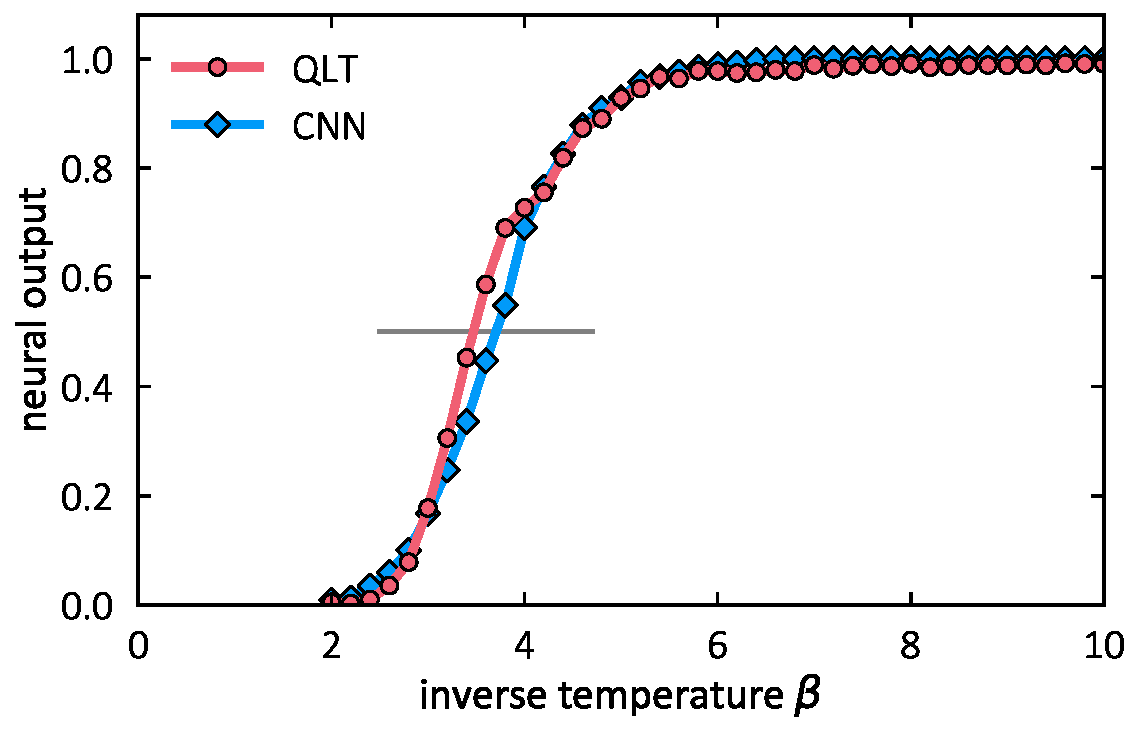
\includegraphics[scale=.43]{fig1.pdf}
\caption{
{\bf Negative-U Hubbard model.} The neural outputs of the quantum loop topography (QLT) and convolutional neural network (CNN) architectures for superconducting transport versus the inverse temperature $\beta$. While the inputs for the deep CNN are the unprocessed Green's functions $P(r,r')$ from the square-lattice negative $U$ Hubbard model in Eq.~\eqref{eq:hubbard}, we pre-process the input for the shallow ANN of the QLT architecture in the form of the quantum loops in Eq.~\eqref{eq:triangle} and \ref{eq:quad}. Both architectures are trained with samples at low temperature $\beta=20$ representing superconducting transport and high temperature $\beta=2$ representing normal state transport. Then the resulting architectures are applied towards the interpolating temperatures. $U=-8$, $\left\langle n\right\rangle= \left\langle n_\uparrow\right\rangle+\left\langle n_\downarrow\right\rangle\simeq 0.9$, $d_c=2$, and the system size is $8\times 8$. }\label{fig:hubbard}
\end{figure}


\begin{figure}
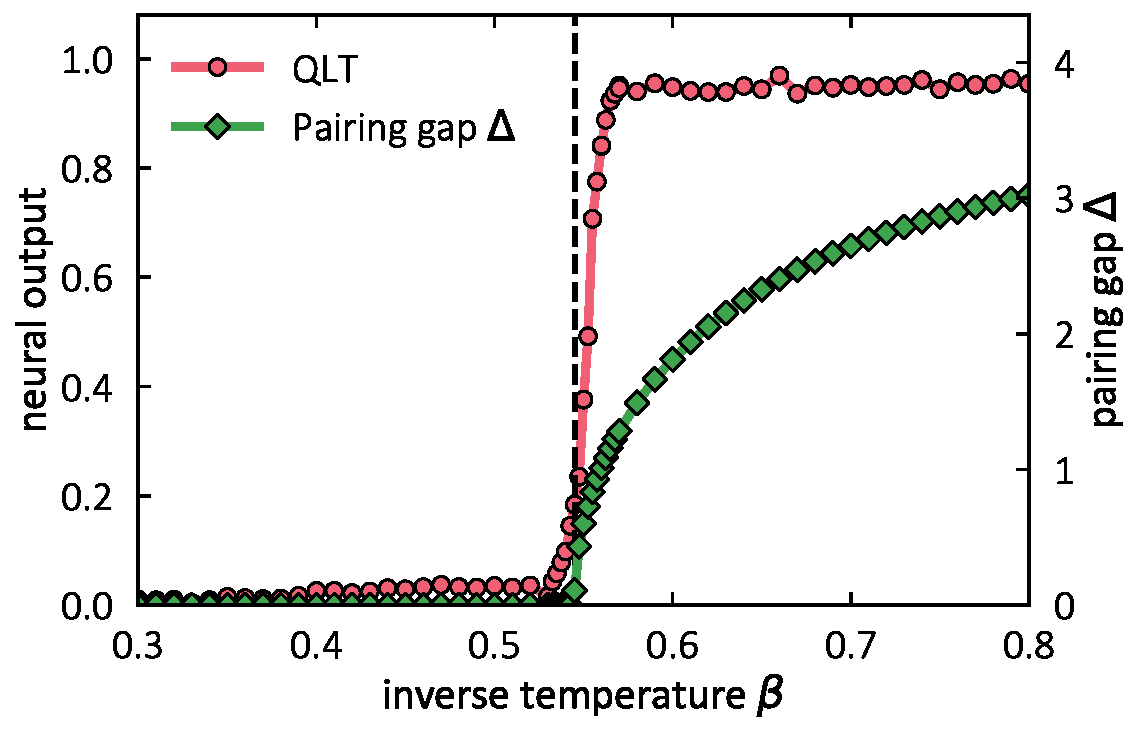
\includegraphics[scale=.43]{fig2.pdf}
\caption{{\bf Mean field theory of the Negative-U Hubbard model.} The mean-field $s$-wave pairing gap $\Delta$ follows the self-consistent gap equation at an inverse temperature $\beta$. The neural output from the QLT architecture is consistent with the debut of the superconducting gap. Here, we obtain the samples of the Green's function $P(r, r')$ through finite-temperature Monte Carlo calculations. $U=-8$, $\mu=-0.5$. The transition temperature $\beta_c\sim 0.545$ is shown as the vertical dashed line. A higher resolution is imposed near $\beta_c$ for clarity.}\label{fig:mlmft}
\end{figure}


% The other architecture we consider is a state-of-the-art deep convolutional neural network (CNN). Such CNN has succeeded in identifying phases and locating phase transitions in quantum many-fermion systems based on raw samples of the Green's functions\cite{Simon2016} without preprocessing. 
 % The neural network consists of two sets of convolutional and max pooling layers followed by two fully-connected layers separated by a dropout layer. The neurons in the final layer has a softmax activation function, while all other neurons are set to be rectified linear units.

%This observation is also consistent with the performance of the neural network on mean-field ansatz, where the superconducting transport onset as soon as a mean-field pairing gap opens. For instance, 

Secondly, we bench-marked the QLT+QMC by comparing ANN assessment of superconductivity against exact results on the the mean field theory of the negative $U$ Hubbard model in Eq.~\eqref{eq:hubbard}. Since mean field theory cannot capture fluctuations the onset of superfluid density and superconducting transition coincide within mean-field theory. Hence we anticipated ANN assessment of superconductivity to be onset at the mean field transition. To test this,  we solved the self-consistent gap equations at  each inverse temperature $\beta$ to obtain the 
 $s$-wave pairing gap $\Delta(\beta)$. We then sampled QLT through finite-temperature Monte Carlo calculations, using the corresponding BdG mean-field model with the respective $\Delta(\beta)$ to generate the quasi-particle occupation number.
 The resulting phase diagram for $U=-8$ and $\mu=-0.5$
 using $\beta=0.3$ and $\beta=0.8$ as the high and  low temperature limit training points are shown in Fig. \ref{fig:mlmft}. \footnote{The training points were chosen to enclose the known mean-field transition point.}
 Indeed, ANN assessment of superconductivity shows a sharp onset at the mean-field superconducting transition.

 Armed with the above results establishing our confidence on QLT+QMC, we now turn to a model in which superconductivity arises from the quantumm critical fluctuations rather than from a hand-picked interaction. Specifically we consider 
 a spin-fermion model in which two flavors of spin$-1/2$ fermions $\psi_x$ and $\psi_y$ are coupled to an easy-plane SDW order parameter $\vec{\varphi}$ at wave vector $\vec Q=(\pi, \pi)$ on a two-dimensional square lattice~\cite{Erez2016}:
\begin{eqnarray}
L&=&L_F+L_\varphi \nonumber\\
L_F &=&  -\sum_{\left\langle ij \right\rangle, s, \alpha} t_{\alpha ij} \psi_{\alpha is}^\dagger \psi_{\alpha js} + \sum_{i, s, \alpha} \psi_{\alpha is}^\dagger \left(\partial_\tau - \mu \right)\nonumber \\
& & +\lambda \sum_{i,s,s'} e^{i \vec Q\cdot \vec r_i} \left[ \vec s\cdot \vec \varphi_i\right]_{ss'} \psi_{xis}^\dagger \psi_{yis'} \nonumber\\
L_\varphi &=& \sum_i \frac{1}{2c^2} \left(\frac{d\vec\varphi_i}{d\tau}\right)^2 + \frac{r}{2}\vec \varphi_i^2 + \frac{u}{4} (\vec \varphi_i^2)^2 \nonumber \\
& & +\frac{1}{2}\sum_{\left\langle ij \right\rangle} (\vec \varphi_i - \vec \varphi_j)^2 \,,
\label{eq:afmetal}
\end{eqnarray}
where $\alpha=x,y$ labels the two fermion flavors, and $s = \uparrow, \downarrow$ denotes the spin. The fermion hopping amplitudes are $t_{x,i,i\pm\hat x}=t_{y,i,i\pm\hat y}=1$ and $t_{x,i,i\pm\hat y}=t_{y,i,i\pm\hat x}=0.5$, and we set the Yukawa coupling $\lambda=3$ and chemical potential $\mu=0.5$. The dynamics of the SDW order parameter is characterized by $r=10.35$ and $u=1$ and the bare bosonic velocity $c=2$. We also set the system size to $8\times 8$. Again we compare the assessments of the CNN on the unprocessed Green's functions to the assessments of the simple ANN on the QLT. 



\begin{figure}
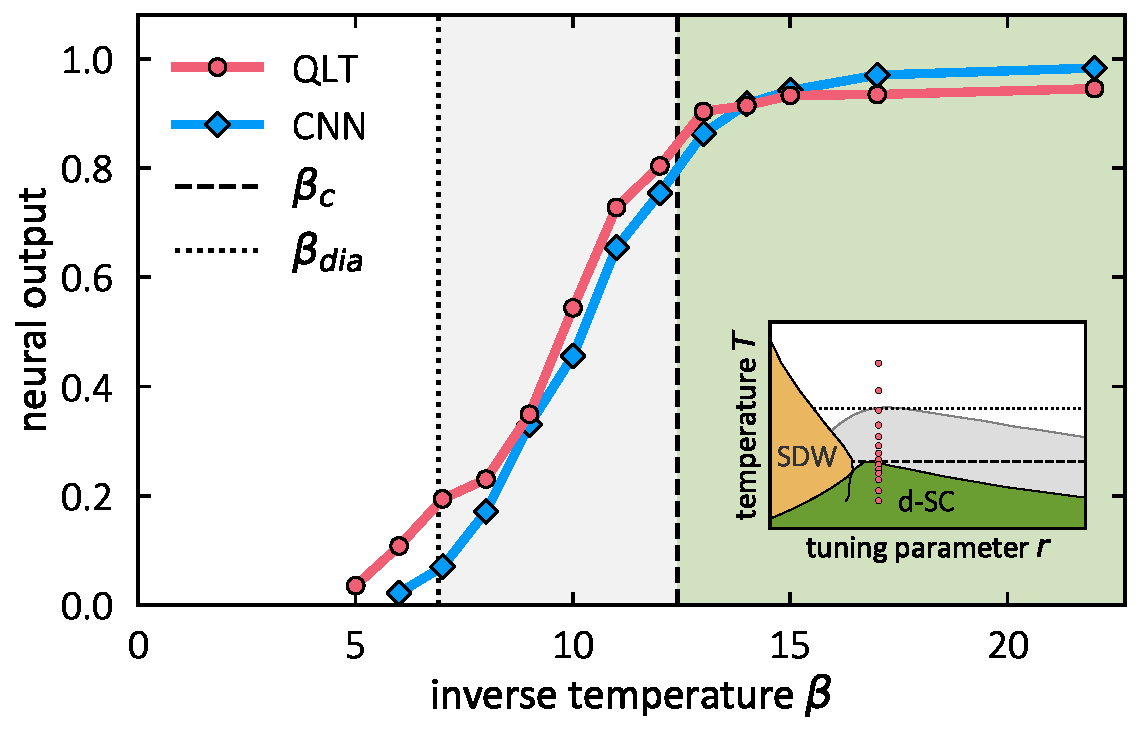
\includegraphics[scale=.43]{fig3.pdf}
\caption{Neural network output for the superconducting transition near a {\bf metallic quantum critical point}. The training points were at $\beta=30$ for superfluid transport and $\beta=5$ for metallic transport.
The vertical lines indicate the superconducting transition temperature $\beta_c\sim 12.5$ (dashed) derived from the superfluid density measurements and the onset of diamagnetic fluctuations $\beta_{dia} \sim 6.9$ (dotted) where the orbital magnetic susceptibility changes sign\cite{Erez2016}.Statistics from 10 different neural networks is shown for the QLT architecture.}
\label{fig:afmetal}
\end{figure}

The results shown in Fig. \ref{fig:afmetal} confirms that QLT+QMC can indeed correctly detect onset of superconducting fluctuations in fermions coupled to quantum critical fluctuations. This is evident in the fact that the neural network output is turning on where the earlier study of current-current correlation found the onset of diagmgnetic fluctuations (dotted line) following the standard approach\cite{Erez2016}. Again the QLT+QMC is arriving at the assessment that is consistent with the CNN assessments albeit using only a fraction ($D/L^2$ where $D$ is the size of the largest loop and $L$ is linear dimension of the system) of data using much simpler ANN.
Note that QLT+QMC achieved the above detection of superconducting transport with only $\sim O(10)$ uncorrelated Monte Carlo steps\footnote{This includes the steps needed in constructing the quantum loops as well as the multiple tests to streamline the accuracy.}, a huge reduction over the required samples necessary in order to follow the standard QMC measurements of the superfluid density\cite{Hong2016, Erez2016}. 



%%%%%%%%%%%%%%%%%%%%%%%%%%%%%%%%%%%%%%%%%%%%%%%%%%%%%%%%%%%%%%%%%%

%\section{Conclusions} 
\noindent{\em Conclusions.-- }
%
To summarize, we have introduced a feature selection protocol for machine learning guided by the response theory in order to target longitudinal transport: the QLT for longitudinal transport. We have show-cased the effectiveness and efficiency of this QLT+QMC approach by employing the approach to models that are known to have superconductivity in their phase diagram. At one level, we showed that the response theory guided QLT+QMC approach performs as well as the much more involved CNN approach rooted in the image recognition techniques. The advantage of QLT+QMC approach is that quantum statistical physics tradition is incorporated into the approach; this synergy simultaneously gives accountability and efficiency to the machine learning. At another level, we showed that the QLT+QMC approach can detect correctly transport signatures of superconducting fluctuation by comparing the neural network outcome to rigorous traditional measurements of the superfluid density. The benefit of QLT+QMC approach for detecting superconducting fluctuation is that its computational cost is considerably lower. Moreover, since QLT is semi-locally defined, it does not require transnational symmetry. We anticipate that QLT+QMC will be even more valuable in detecting states without traditional representation that are nevertheless defined through non-trivial transport properties such as non-Fermi liquids. 




%We show that the 'big data' issue can be resolved by either resorting to powerful deep learning mechanisms such as the CNN, or introducing feature-selection interface such as QLT. Our studies further embrace the power of machine learning and open its door to other condensed matter systems.

%The consistency between the results from the CNN and QLT-assisted simple ANN is an interesting example on how we can balance our cost on human intelligence and artificial intelligence. We note that the QLT samples are obtained from the raw samples of the Green's functions, so the latter is equally inclusive if not more; on the other hand, QLT's pre-processing of the data involves non-linear chain products of the raw Green's function data, therefore, if the QLT data is indeed sufficient for determining the emergent superconductivity, starting from the raw Green's functions may invoke extra redundancy and logical steps. This requirement can be compensated by powerful deep neural networks such as the CNN. We advise choosing between deeper neural network and feature-selection layers depending on the amount theoretical understanding and intuition on the target systems as well as computational resources. 

%In addition, our work also features thermal phase transitions between superconductors and normal metals in two dimensions of Kosterlitz-Thouless character where machine learning ansatz saw substantial subtlety and difficulty previously\cite{Anna2018}. 



%%%%%%%%%%%%%%%%%%%%%%%%%%%%%%%%%%%%%%%%%%%%%%%%%%%%%%%%%%%%%%%%%%

\vskip 2cm

{\it Acknowledgement --} 
We acknowledge useful discussions with Erez Berg, Yi-Ting Hsu, and Hong Yao. YZ and E-AK acknowledge the support from the U.S. Department of Energy, Office of Basic Energy Sciences, Division of Materials Science and Engineering under Award DE-SC0018946.
The Cologne group acknowledges partial support from the DFG collaborative research center TR 183 (project B01). 
The numerical simulations were performed on the JUWELS cluster at FZ J\"ulich and the CHEOPS cluster at RRZK Cologne.


%\bibliographystyle{apsrev4-1}
\bibliography{refs,t+X-NSF}
%\newpage
\appendix

\section{Current-current correlations and quantum loop topography}

In this appendix, we explore the connection between the zero-frequency current-current correlation in Eq.~\eqref{eq:Lambda}
\begin{equation}
\left. \begin{aligned}
\Lambda&\left({\bf r}_1, {\bf r}_2;\omega=0\right) = \int d\tau \left\langle \hat{j}_x({\bf r}_1,\tau)\hat{j}_x({\bf r}_2,0) \right\rangle  \\
&=\sum_{n\ne G} \frac{\left\langle G \left| \hat{j}_x({\bf r}_1)  \left|n\left\rangle  \right\langle n\right| \hat{j}_x({\bf r}_2)\right| G\right\rangle}{E_n-E_G} 
\end{aligned}
\right.
\end{equation}
and the products of two-point correlators trailing loops, especially in the presence of superconductivity. For simplicity, we focus on a mean-field Hamiltonian with a flat band $\hat{H}'=1/2-\hat P$, $\hat P=\sum_{{\bf r}'{\bf r}}P_{{\bf r}'{\bf r}}a^\dagger_{{\bf r}'} a_{\bf r}=\sum_{\mu}a^\dagger_\mu a_\mu$. Then, 
\begin{equation}
\left. \begin{aligned}
\Lambda\left({\bf r}_1, {\bf r}_2;\omega=0\right)&
=\sum_{\mu, \nu}\left\langle \mu \left| \hat{j}_x({\bf r}_1)  \left|\nu\left\rangle  \right\langle \nu\right|\hat{j}_x({\bf r}_2)\right| \mu\right\rangle \\
= \mbox{tr}&\left[\hat{P} \hat{j}_x({\bf r}_1) \left(1-\hat{P}\right) \hat{j}_x({\bf r}_2)\right]
\end{aligned}
\right.
\label{eq:app1}
\end{equation}
where $\left|\mu\right\rangle$ ($\left|\nu\right\rangle$) are the single-particle states that are occupied (empty) in the ground state $\left|G\right\rangle$ of $\hat{H}'$. It follows that $\epsilon_\mu=-1/2$, $\epsilon_\nu=1/2$, and $1-\hat P=\sum_{\nu}a^\dagger_\nu a_\nu=\sum_{\nu}\left|\nu\right\rangle\left\langle\nu\right|$. We note that the arguments also apply for a mean-field Bogoliubov deGenne Hamiltonian of a superconductor
\begin{equation}
\left. \begin{aligned}
\hat{H}_{BdG} & =  \sum_{\bf{r}'\bf{r}}t_{\bf{r}'\bf{r}}c_{\bf{r}'}^{\dagger}c_{\bf{r}}+\Delta_{\bf{r}'\bf{r}}c_{\bf{r}'}^{\dagger}c_{\bf{r}}^{\dagger}+\mbox{h.c.}\\
=\frac{1}{2}\sum_{\bf{r}'\bf{r}}&t_{\bf{r}'\bf{r}}\left(a_{\bf{r}'}^{\dagger}a_{\bf{r}}-\tilde{a}_{\bf{r}}^{\dagger}\tilde{a}_{\bf{r}'}\right)
+\Delta_{\bf{r}'\bf{r}}\left(a_{\bf{r}'}^{\dagger}\tilde{a}_{\bf{r}}-a_{\bf{r}}^{\dagger}\tilde{a}_{\bf{r}'}\right)+\mbox{h.c.}
\end{aligned},
\right.
\end{equation}
where $a_{\bf{r}}^\dagger=\tilde{a}_{\bf{r}}=c_{\bf{r}}^\dagger$ is the creation operator of the original electrons. With the new basis of both the electron and hole operators $a$ and $\tilde{a}$, the Hamiltonian $\hat{H}_{BdG}$ again takes a fermion bi-linear form. In the following, we will drop the tilde and denote $a(\bf{r})$ and $\tilde{a}(\bf{r})$ with their respective electric charge $q=\pm 1$ that we contain in the label $\bf{r}$.

Commonly, the $\vec{x}$-direction current operator at position ${\bf r}$ is $\hat{j}_x({\bf r})=-i\left[\hat{H}'({\bf r}),\hat x\right]=\sum_{{\bf r}'}iP_{{\bf r}'{\bf r}}c_{{\bf r}'}^\dagger c_{{\bf r}}\left(x-x'\right)+\mbox{h.c.}$, where $x$ is the $\vec{x}$-direction component of ${\bf r}$. In the case of Bogoliubov deGenne Hamiltonian, however, we need to incorporate the sign of the charge and generalize the current operator as ${\bf r}$ is $\hat{j}_x({\bf r})=-\frac{i}{2}\left(\hat{q}\left[\hat{H}'({\bf r}),\hat x\right]+\left[\hat{H}'({\bf r}),\hat x\right]\hat{q}\right)$. Putting this into Eq.\ref{eq:app1}, we have :
\begin{equation}
\left.
\begin{aligned}
\mbox{tr}&\left[\hat{P} \hat{j}_x({\bf r}_1) \left(1-\hat{P}\right) \hat{j}_x({\bf r}_2)\right]  \\
=& \frac{1}{4} \sum_{{\bf r}_3 {\bf r}_4 {\bf r}'_1 {\bf r}'_2{\bf r}'_3{\bf r}'_4}P_{{\bf r}'_4 {\bf r}_4}P_{{\bf r}'_1{\bf r}_1}\left(P_{{\bf r}'_3{\bf r}_3}-\delta_{{\bf r}'_3{\bf r}_3}\right)P_{{\bf r}'_2{\bf r}_2} \\&\times\left(x_1-x'_1\right)\left(x_2-x'_2\right)\left(q_1+q'_1\right)\left(q_2+q'_2\right)
\\&\times\left\langle0\left|a_{{\bf r}_4}a^\dagger_{{\bf r}'_1} a_{{\bf r}_1} a^\dagger_{{\bf r}'_3} a_{{\bf r}_3} a^\dagger_{{\bf r}'_2} a_{{\bf r}_2} a^\dagger_{{\bf r}'_4}\right|0\right\rangle \\
=& \sum_{{\bf r}_3 {\bf r}_4}P_{{\bf r}_2 {\bf r}_4}P_{{\bf r}_4{\bf r}_1}P_{{\bf r}_1{\bf r}_3}P_{{\bf r}_3{\bf r}_2}\\
&\times\left(x_1-x_4\right)\left(x_2-x_3\right)\left(q_1+q_4\right)\left(q_2+q_3\right)/4 \\
 &- \sum_{{\bf r}_4}P_{{\bf r}_2 {\bf r}_4}P_{{\bf r}_4{\bf r}_1}P_{{\bf r}_1{\bf r}_2}\\
 &\times\left(x_1-x_4\right)\left(x_2-x_1\right)\left(q_1+q_4\right)\left(q_2+q_1\right)/4
\label{eq:app2}\end{aligned}\right.
\end{equation}

On the other hand, the expectation value of the two-point correlator is given by:
\begin{equation}
\left. \begin{aligned}
\left\langle a_{{\bf r}'}^{\dagger}a_{{\bf r}}\right\rangle  &= \sum_{\mu}\left\langle \mu|a_{{\bf r}'}^{\dagger}a_{{\bf r}}|\mu\right\rangle \\
  =\sum_{\tilde{{\bf r}}' \tilde{{\bf r}}}&P_{\tilde{{\bf r}}\tilde{{\bf r}}'}\left\langle 0|a_{\tilde{{\bf r}}'}a_{{\bf r}'}^{\dagger}a_{{\bf r}}a_{\tilde{{\bf r}}}^{\dagger}|0\right\rangle  =P_{{\bf r}{\bf r}'}
\end{aligned}\right. 
\label{eq:j-jbdg}
\end{equation}
Therefore, Eq.~\eqref{eq:app2} can be expressed in terms of products of two-point correlators trailing triangles and quadrilaterals. In particular, in terms of the original electron correlators $P_{\bf{r}\bf{r}'}=\left\langle c^\dagger_{\bf{r}}c_{\bf{r}'} \right\rangle$, $q_{\bf{r}}=1$ for all and Eq.~\eqref{eq:j-jbdg} returns to Eq.\ref{eq:j-j}. 

%This is Mean field theory discussion. No longer necessary. 

%\section{Derivation of the real-space formulation of $\Lambda'_{xx}$}


%In addition, since the quasi-particles are no longer necessarily electron-like, care should be taken upon defining the current density operator (along the $\hat x$ direction): $j_x (q_y)= \left\{Q, v_x\right\} e^{iq_y y}/2$, where $v_x = i\left[H, x\right]$ is the $\hat x$ direction velocity operator and $Q$ is the charge operator that . and the trace in $L_{ijkl}$ ($L'_{jkl}$) is over the spin up and spin down electrons $c^\dagger_\uparrow$, $c^\dagger_\downarrow$ as well as the holes $c_\uparrow$, $c_\downarrow$ for a given set of sites $ijkl$ ($jkl$)
%Note that the transformation $c^\dagger_{\vec r,\downarrow} \rightarrow (-1)^{x+y} c_{\vec r,\downarrow}$ maps $U$ to $-U$ in Eq.~\eqref{eq:hubbard} and $H^{BCS}_{MF}$ to $H^{SDW}_{MF}$ in Eq.~\eqref{eq:mfham}, and vice versa. Such equivalence in $L$ and $L'$ between the two phases, however, is broken by the charge operator $Q$, which changes sign after the transformation. Indeed, the static paramagnetic current-current correlation function $\Lambda_{xx}$ and that for the corresponding $H'=-P$ are shown in Fig. \ref{fig:exact}. 

%Scalapino, White and Zhang\cite{Scalapino1993} have shown from a response theory perspective that there are two contributions to $D_s/e^2$, a diamagnetic one $\langle-k_x\rangle$ related to the $\hat x$ direction kinetic energy density, and the static paramagnetic current-current correlation function $\Lambda_{xx}(q_x=0, q_y\rightarrow 0)$. Counter-intuitively, the diamagnetic part $\langle-k_x\rangle$ exists not only in superconductors, but also in normal metals or insulators, and it is rather the paramagnetic part that makes the distinction - while it cancels the diamagnetic part $\langle-k_x\rangle$ in the latter case, it vanishes in a superconductor thus exposing the real diamagnetic Meissner effect\footnote{The exception is a band that is initially fully occupied, where both diamagnetic and paramagnetic contributions vanish whatsoever; however, such a trivial band insulator is uninteresting and can be excluded from superconductivity in the first place.}:

%We must insert the charge operator $Q$ obeys $Qc^\dagger = c^\dagger$ and $Qc=-c$ between the Green's functions that make up the QLT operators.

%\begin{eqnarray}
%\Lambda'_{xx} &=& \frac{1}{N}\underset{q_y\rightarrow 0}{\lim}  \mbox{tr} \left[ P  j_x(-q_y)  \left(1-P\right) j_x(q_y)\right] \nonumber\\
%&=& \frac{1}{N}\underset{q_y\rightarrow 0}{\lim}\underset{ijkl}{\sum} L_{ijkl}\times \left(x_i-x_j\right)\left(x_k-x_l\right)e^{iq_y(y_l-y_j)} \nonumber\\
%& & - \underset{jkl}{\sum} L'_{jkl}\times \left(x_j-x_k\right)\left(x_k-x_l\right)e^{iq_y(y_l-y_k)}
%\label{eq:Lambdaprime}
%\end{eqnarray}
%where
%\begin{eqnarray}
%L_{ijkl}&=&\frac{1}{4}\mbox{tr} \left[P_{ij} \{Q, P_{jk}\} P_{kl} \{Q,P_{li}\}\right]\nonumber\\
%L'_{jkl}&=&\frac{1}{4}\mbox{tr} \left[P_{jk}\{Q,P_{kl}\}\{Q,P_{lj}\}\right]
%\label{eq:qls2}
%\end{eqnarray}

%\begin{figure}
%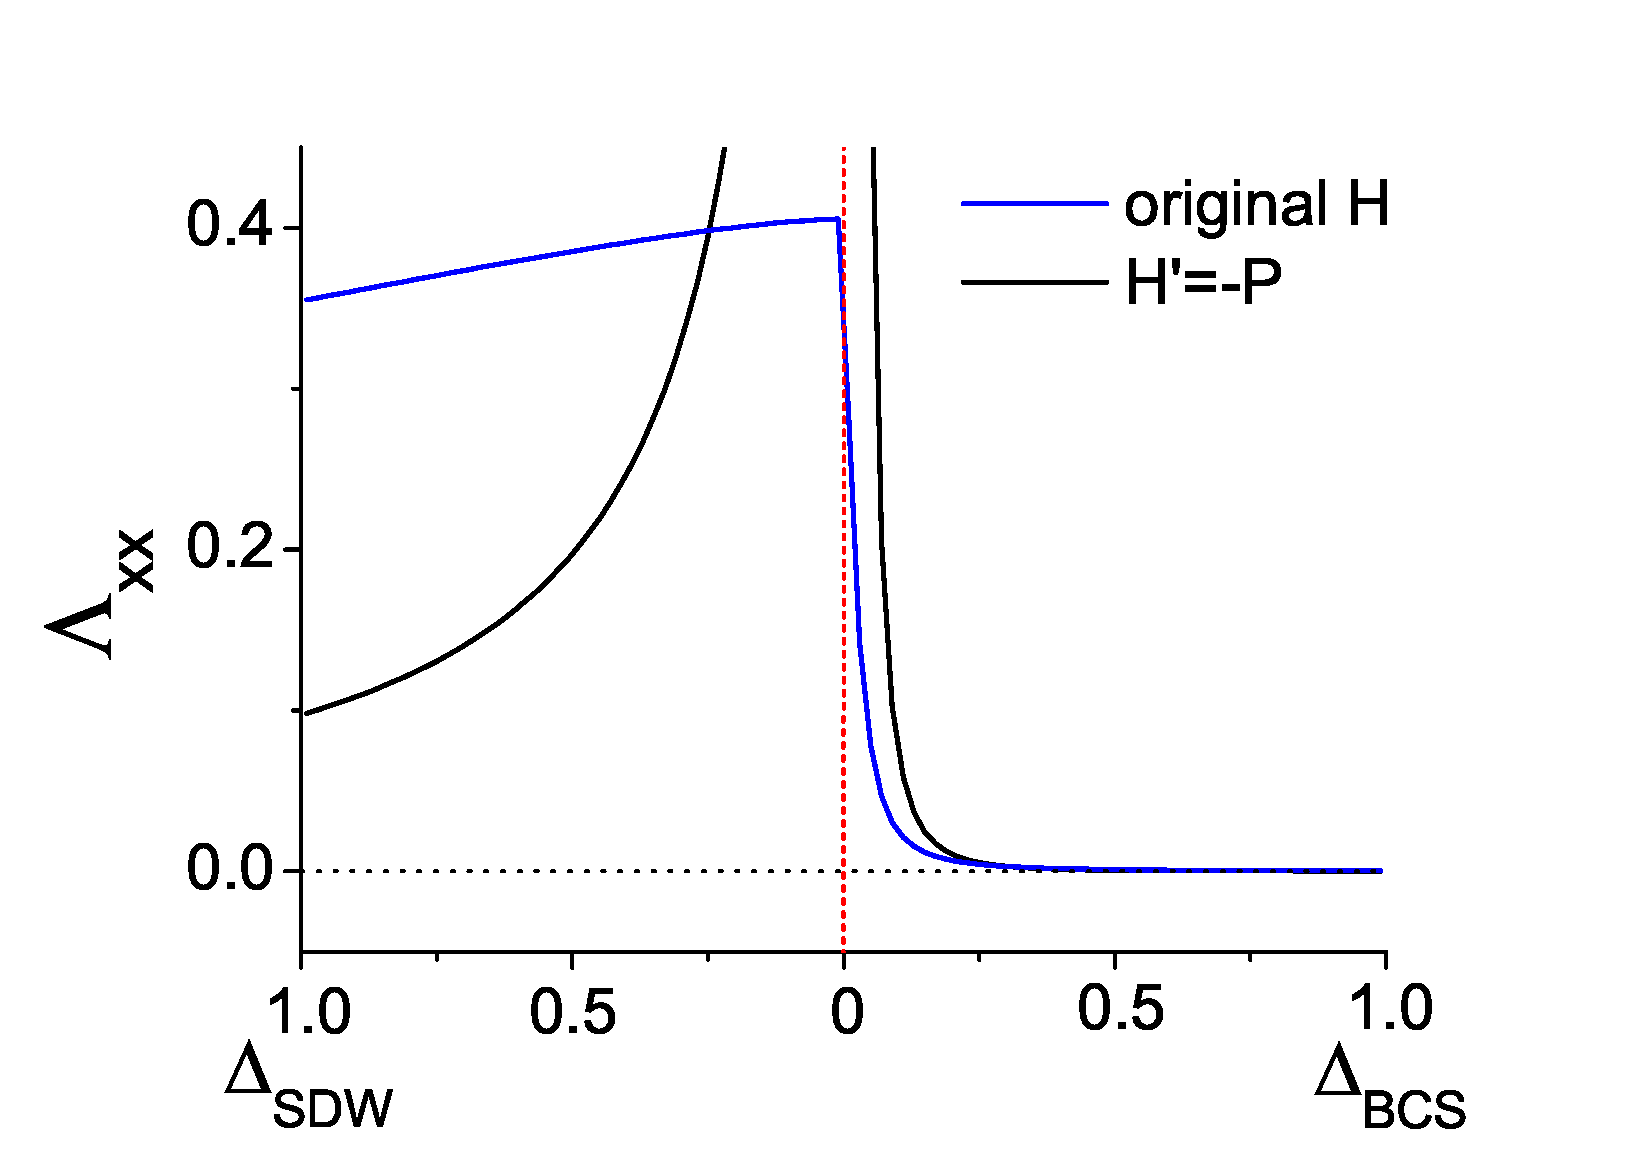
\includegraphics[scale=0.35]{figkLambda.eps}
%\caption{Static paramagnetic current-current correlation function $\Lambda_{xx}(q_x=0, q_y\rightarrow 0)$ as in Eq.~\eqref{eq:lambdaform} for the original mean-field Hubbard model at half filling on two-dimensional square lattice in Eq.~\eqref{eq:mfham} and the phase-equivalent effective model $H'=-P$. The vertical red dashed line where $\Delta_{BCS}=\Delta_{SDW}=0$ is the mean-field phase boundary between the SDW insulator and the superconductor. In comparison with the original Hamiltonian, $H'$ does induce significant quantitative changes to $\Lambda_{xx}$; however, the phase-defining qualitative feature remains intact: $\Lambda_{xx}$ vanishes rapidly in a superconducting phase consistent with the onset of the Meissner effect.}\label{fig:exact}
%\end{figure}

%We consider instead an alternative model described by $H'=-P$,  where $P = \underset{n}{\sum} |n\rangle\langle n|$ is the projection operator onto the ground state. $H'$ shares with $H$ the same group of occupied (unoccupied) states $\left|n\right\rangle$ ($\left|m\right\rangle$) yet with a flattened quasiparticle spectrum $E'_n=-1$ ($E'_m=0$). Since we expect $H'$ to be superconducting if and only if $H$ is superconducting and the two models are adiabatically connected without closing the spectrum gap, we can based our judging criteria of the Meissner effect upon $\Lambda'_{xx}$ instead of $\Lambda_{xx}$, see Fig. \ref{fig:exact}. 

%\begin{eqnarray}
%\Lambda'_{xx}&=&-\underset{q_y\rightarrow 0}{\lim} \mbox{tr} \left[P \left\{Q,\left[H', x\right]\right\} \exp(-iq_y y)(1-P) \left\{Q,\left[H', x\right]\right\}\exp(iq_y y)\right] 
%\end{eqnarray}

%\begin{eqnarray}
%\Lambda'_{xx} &=& \underset{q_y\rightarrow 0}{\lim}\mbox{tr} \left[ P  j_x(-q_y)  \left(1-P\right) j_x(q_y)\right] \\
%&=& \underset{ijkl}{\sum} L_{ijkl}\times %\left(x_i-x_j\right)\left(x_k-x_l\right)\underset{q_y\rightarrow 0}{\lim}\exp\left[iq_y(y_l-y_j)\right] \nonumber\\
%&-&\underset{jkl}{\sum} L'_{jkl}\times \left(x_j-x_k\right)\left(x_k-x_l\right)\underset{q_y\rightarrow 0}{\lim}\exp\left[iq_y(y_l-y_k)\right]\nonumber
%\end{eqnarray}

\end{document}
